%% LyX 2.0.5.1 created this file.  For more info, see http://www.lyx.org/.
%% Do not edit unless you really know what you are doing.
\documentclass{article}\usepackage{graphicx, color}
%% maxwidth is the original width if it is less than linewidth
%% otherwise use linewidth (to make sure the graphics do not exceed the margin)
\makeatletter
\def\maxwidth{ %
  \ifdim\Gin@nat@width>\linewidth
    \linewidth
  \else
    \Gin@nat@width
  \fi
}
\makeatother

\IfFileExists{upquote.sty}{\usepackage{upquote}}{}
\definecolor{fgcolor}{rgb}{0.2, 0.2, 0.2}
\newcommand{\hlnumber}[1]{\textcolor[rgb]{0,0,0}{#1}}%
\newcommand{\hlfunctioncall}[1]{\textcolor[rgb]{0.501960784313725,0,0.329411764705882}{\textbf{#1}}}%
\newcommand{\hlstring}[1]{\textcolor[rgb]{0.6,0.6,1}{#1}}%
\newcommand{\hlkeyword}[1]{\textcolor[rgb]{0,0,0}{\textbf{#1}}}%
\newcommand{\hlargument}[1]{\textcolor[rgb]{0.690196078431373,0.250980392156863,0.0196078431372549}{#1}}%
\newcommand{\hlcomment}[1]{\textcolor[rgb]{0.180392156862745,0.6,0.341176470588235}{#1}}%
\newcommand{\hlroxygencomment}[1]{\textcolor[rgb]{0.43921568627451,0.47843137254902,0.701960784313725}{#1}}%
\newcommand{\hlformalargs}[1]{\textcolor[rgb]{0.690196078431373,0.250980392156863,0.0196078431372549}{#1}}%
\newcommand{\hleqformalargs}[1]{\textcolor[rgb]{0.690196078431373,0.250980392156863,0.0196078431372549}{#1}}%
\newcommand{\hlassignement}[1]{\textcolor[rgb]{0,0,0}{\textbf{#1}}}%
\newcommand{\hlpackage}[1]{\textcolor[rgb]{0.588235294117647,0.709803921568627,0.145098039215686}{#1}}%
\newcommand{\hlslot}[1]{\textit{#1}}%
\newcommand{\hlsymbol}[1]{\textcolor[rgb]{0,0,0}{#1}}%
\newcommand{\hlprompt}[1]{\textcolor[rgb]{0.2,0.2,0.2}{#1}}%

\usepackage{framed}
\makeatletter
\newenvironment{kframe}{%
 \def\at@end@of@kframe{}%
 \ifinner\ifhmode%
  \def\at@end@of@kframe{\end{minipage}}%
  \begin{minipage}{\columnwidth}%
 \fi\fi%
 \def\FrameCommand##1{\hskip\@totalleftmargin \hskip-\fboxsep
 \colorbox{shadecolor}{##1}\hskip-\fboxsep
     % There is no \\@totalrightmargin, so:
     \hskip-\linewidth \hskip-\@totalleftmargin \hskip\columnwidth}%
 \MakeFramed {\advance\hsize-\width
   \@totalleftmargin\z@ \linewidth\hsize
   \@setminipage}}%
 {\par\unskip\endMakeFramed%
 \at@end@of@kframe}
\makeatother

\definecolor{shadecolor}{rgb}{.97, .97, .97}
\definecolor{messagecolor}{rgb}{0, 0, 0}
\definecolor{warningcolor}{rgb}{1, 0, 1}
\definecolor{errorcolor}{rgb}{1, 0, 0}
\newenvironment{knitrout}{}{} % an empty environment to be redefined in TeX

\usepackage{alltt}
\usepackage[sc]{mathpazo}
\usepackage{geometry}
\geometry{verbose,tmargin=2.5cm,bmargin=2.5cm,lmargin=2.5cm,rmargin=2.5cm}
\setcounter{secnumdepth}{2}
\setcounter{tocdepth}{2}
\usepackage{url}
\usepackage[unicode=true,pdfusetitle,
 bookmarks=true,bookmarksnumbered=true,bookmarksopen=true,bookmarksopenlevel=2,
 breaklinks=false,pdfborder={0 0 1},backref=false,colorlinks=false]
 {hyperref}
\hypersetup{
 pdfstartview={XYZ null null 1}}
\usepackage{breakurl}
\begin{document}





\title{Stat 2025- HW 3}
\author{Michael Discenza}

\maketitle

I first import the data and conduct some exploratory data analysis 
\begin{knitrout}
\definecolor{shadecolor}{rgb}{0.969, 0.969, 0.969}\color{fgcolor}\begin{kframe}
\begin{alltt}
ToyExample <- \hlfunctioncall{read.table}(\hlstring{"http://www.stat.columbia.edu/~madigan/W2025/data/ToyExample.dat"}, 
    header = TRUE)
\hlfunctioncall{attach}(ToyExample)
\end{alltt}
\end{kframe}
\end{knitrout}

Then I plot the distribution of each predictor for responses y=0 and y=1.  This provides some intuition about how the features might help us differentiate between records that are classfied by 0 and 1.



\begin{knitrout}
\definecolor{shadecolor}{rgb}{0.969, 0.969, 0.969}\color{fgcolor}

{\centering 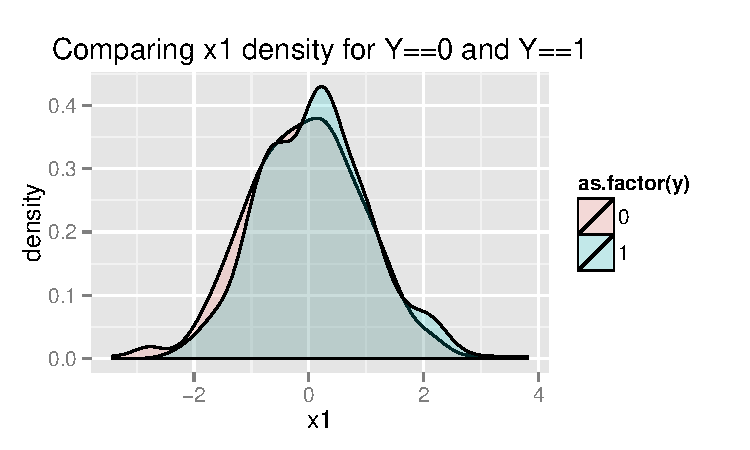
\includegraphics[width=\maxwidth]{figure/minimal-exploratorydataanalysis1} 
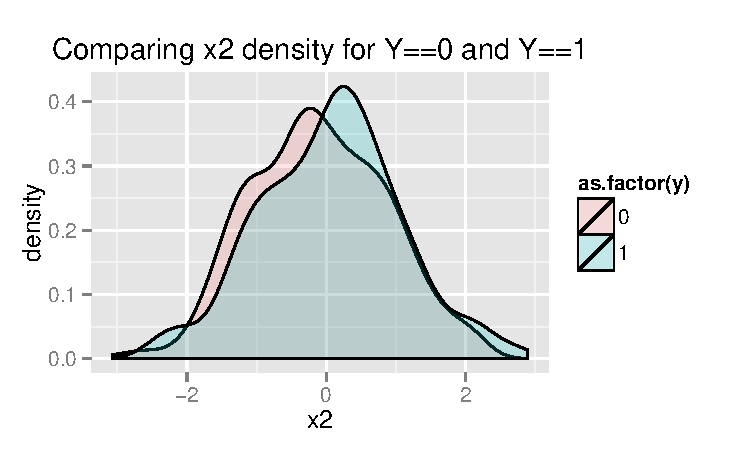
\includegraphics[width=\maxwidth]{figure/minimal-exploratorydataanalysis2} 
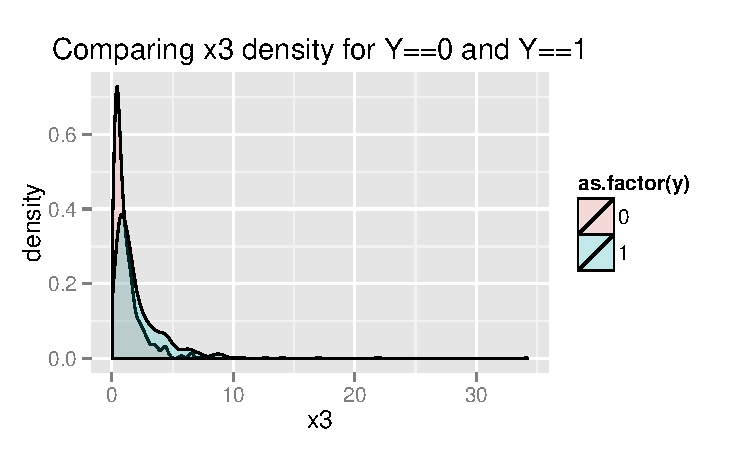
\includegraphics[width=\maxwidth]{figure/minimal-exploratorydataanalysis3} 

}



\end{knitrout}

Before moving into fitting complex logistic regression models with multipl predictors, I fit models with single predictors and examine residual plots to see if there are patterns that indicate a transformation of any of the predictors might be useful.  Instead of plotting the actual data points along y=0 and y=1, I plot the distributions of the x variables along those horizontal lines so that the relationships can be seen more clearly.


\begin{knitrout}
\definecolor{shadecolor}{rgb}{0.969, 0.969, 0.969}\color{fgcolor}\begin{kframe}
\begin{alltt}
testmodel1 <- \hlfunctioncall{glm}(y ~ x1, family = binomial, data = ToyExample)
pred1 <- \hlfunctioncall{predict}(testmodel1, type = \hlstring{"response"})
\hlfunctioncall{par}(mfrow = \hlfunctioncall{c}(1, 2))
\hlfunctioncall{logi.hist.plot}(ToyExample$x1, ToyExample$y, boxp = FALSE, type = \hlstring{"hist"}, col = \hlstring{"gray"}, main = \hlstring{"Fitted Logistic Regression with x1 as Predictor"})
\hlfunctioncall{plot}(testmodel1$residuals ~ ToyExample$x1, main = \hlstring{"Residuals vs. x1"})
\hlcomment{# x2}
testmodel2 <- \hlfunctioncall{glm}(y ~ x2, family = binomial, data = ToyExample)
pred2 <- \hlfunctioncall{predict}(testmodel2, type = \hlstring{"response"})
\hlfunctioncall{par}(mfrow = \hlfunctioncall{c}(1, 2))
\hlfunctioncall{logi.hist.plot}(x2, y, boxp = FALSE, type = \hlstring{"hist"}, col = \hlstring{"gray"}, main = \hlstring{"Fitted Logistic Regression with x2 as Predictor"})
\hlfunctioncall{plot}(testmodel2$residuals ~ ToyExample$x2, main = \hlstring{"Residuals vs. x2"})
\hlcomment{# 3}
testmodel3a <- \hlfunctioncall{glm}(ToyExample$y ~ ToyExample$x3, family = binomial, data = ToyExample)
pred3 <- \hlfunctioncall{predict}(testmodel3a, type = \hlstring{"response"})
\hlfunctioncall{par}(mfrow = \hlfunctioncall{c}(1, 2))
\hlfunctioncall{logi.hist.plot}(ToyExample$x3, ToyExample$y, boxp = FALSE, type = \hlstring{"hist"}, col = \hlstring{"gray"})
\hlfunctioncall{plot}(testmodel3a$residuals ~ ToyExample$x3, main = \hlstring{"Residuals vs. x3"})
\end{alltt}
\end{kframe}

{\centering 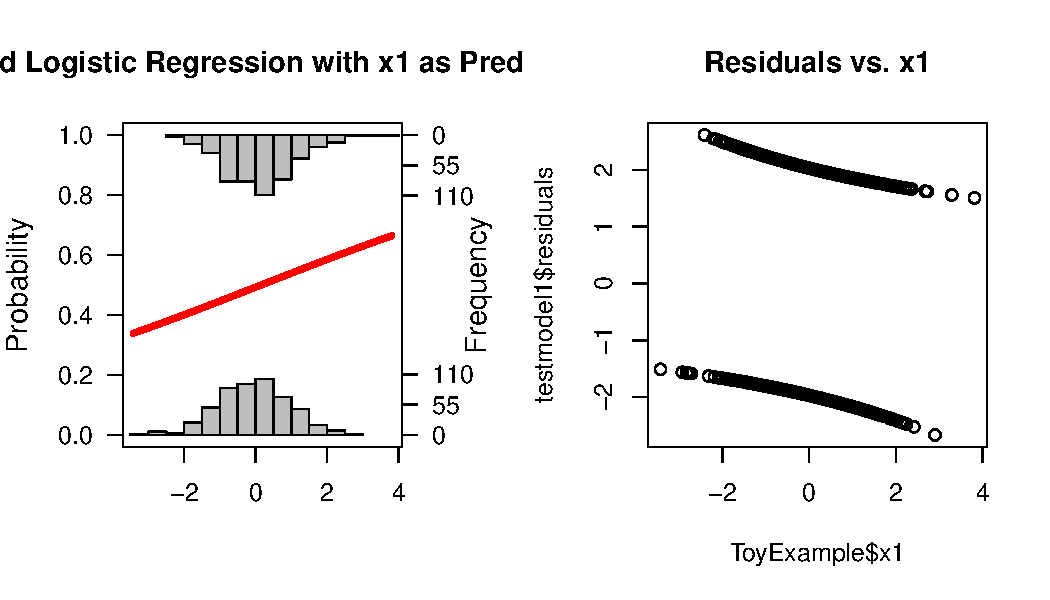
\includegraphics[width=\maxwidth]{figure/minimal-singlevariablemodel1} 
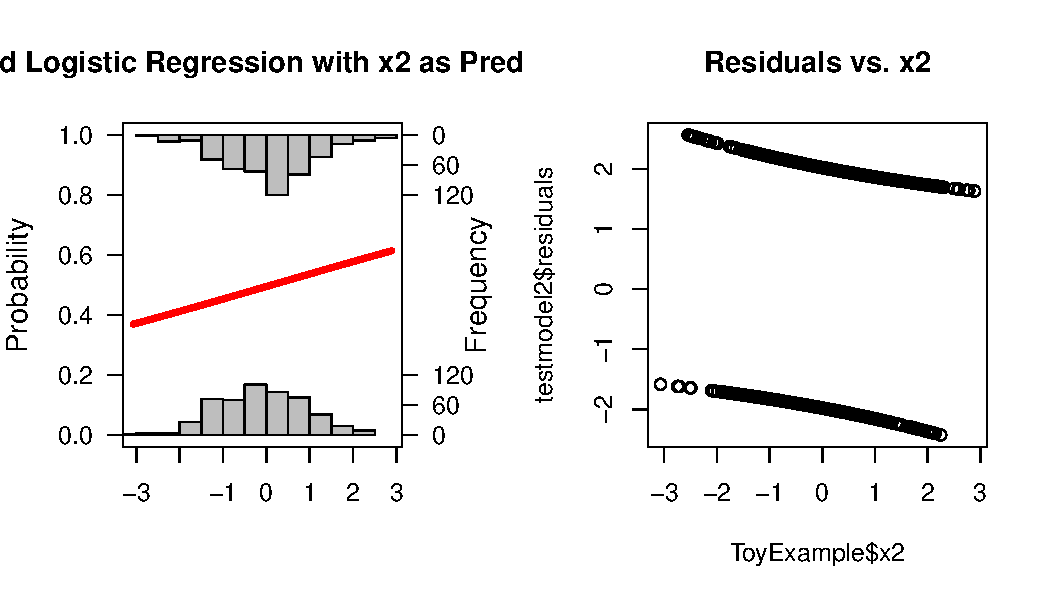
\includegraphics[width=\maxwidth]{figure/minimal-singlevariablemodel2} 
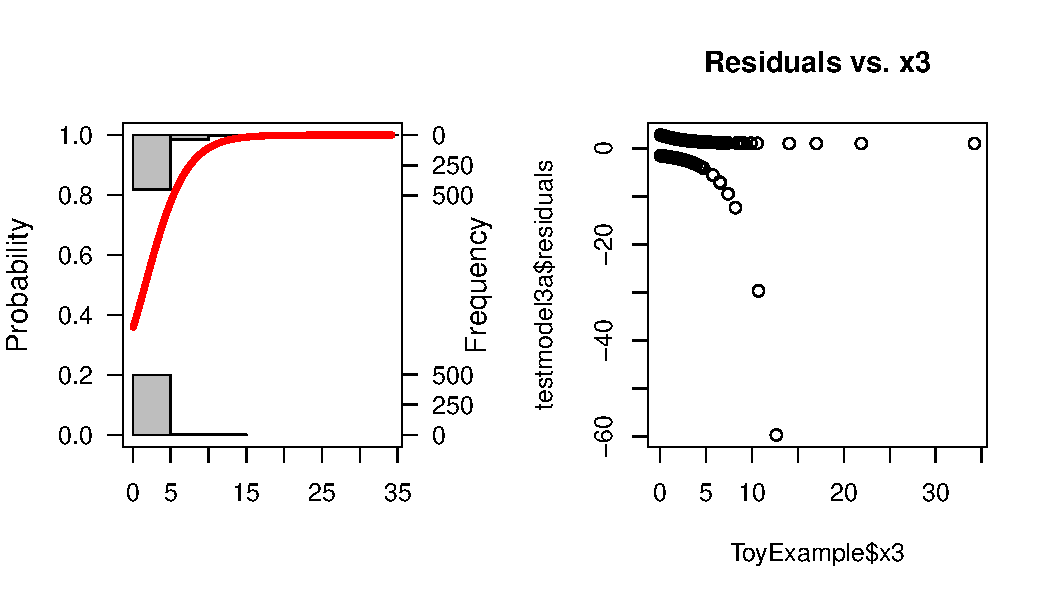
\includegraphics[width=\maxwidth]{figure/minimal-singlevariablemodel3} 

}



\end{knitrout}


We can confirm that there are indeed issues fitting a logistic regression model to x3.  To get rid of the problem with the pattern of the residuals, we transform x3 and instead fit the model to log of x3:
\begin{knitrout}
\definecolor{shadecolor}{rgb}{0.969, 0.969, 0.969}\color{fgcolor}\begin{kframe}
\begin{alltt}
\hlfunctioncall{ggplot}(ToyExample, \hlfunctioncall{aes}(\hlfunctioncall{log}(x3), fill = \hlfunctioncall{as.factor}(y))) + \hlfunctioncall{geom_density}(alpha = 0.2) + \hlfunctioncall{labs}(title = \hlfunctioncall{expression}(\hlstring{"Comparing \hlfunctioncall{log}(x3) density for Y==0 and Y==1"}))
testmodel3b <- \hlfunctioncall{glm}(y ~ \hlfunctioncall{log}(x3), family = binomial, data = ToyExample)
\hlfunctioncall{par}(mfrow = \hlfunctioncall{c}(1, 2))
\hlfunctioncall{logi.hist.plot}(\hlfunctioncall{log}(x3), y, boxp = FALSE, type = \hlstring{"hist"}, col = \hlstring{"gray"})
\hlfunctioncall{plot}(testmodel3b$residuals ~ \hlfunctioncall{log}(x3), main = \hlstring{"Residuals vs. \hlfunctioncall{log}(x3)"})

ToyExample$x3 <- \hlfunctioncall{log}(ToyExample$x3)
\hlfunctioncall{colnames}(ToyExample)[4] <- \hlstring{"logx3"}
\end{alltt}
\end{kframe}

{\centering 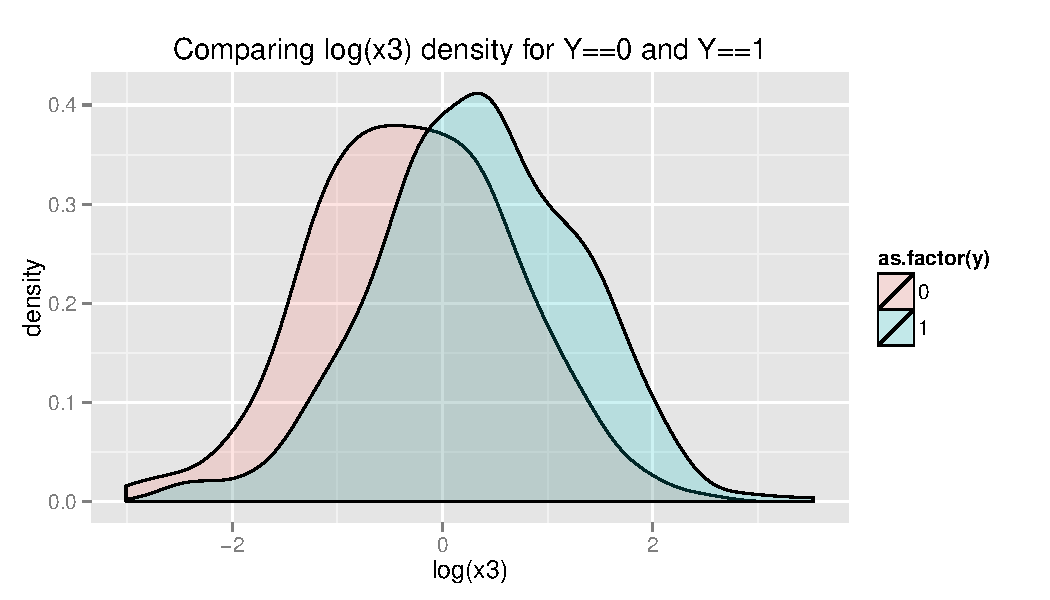
\includegraphics[width=\maxwidth]{figure/minimal-logx31} 
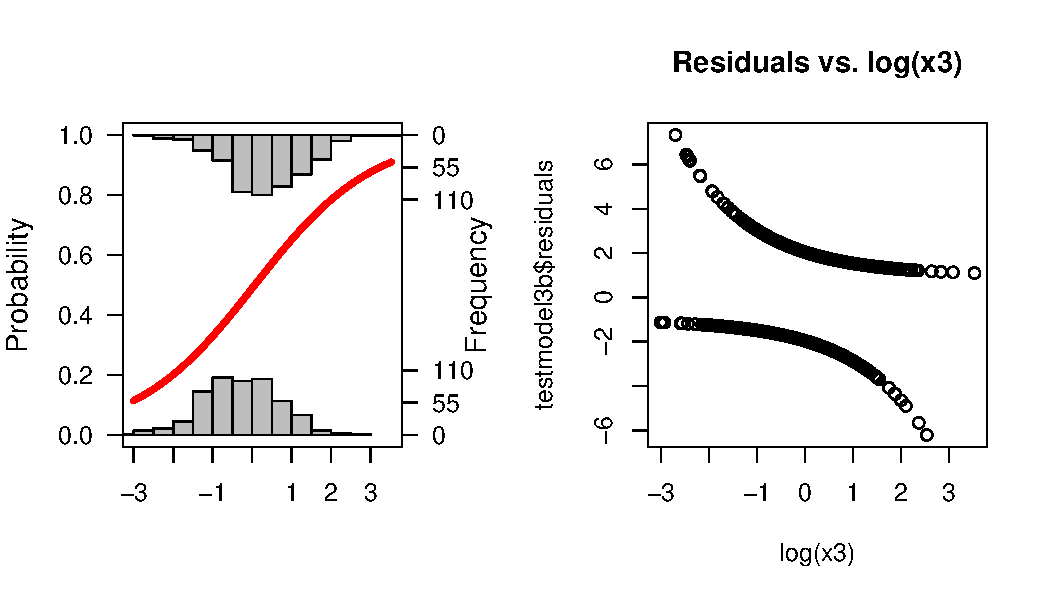
\includegraphics[width=\maxwidth]{figure/minimal-logx32} 

}



\end{knitrout}


Having established that each of the predictors indivdually are acceptable to use in logistic regression, I then proceed to model selection by searching the model space of the combinations of x1, x2, and the log of x3.  To start this procedure, I define functions to enumerate all possible models, fit theses models, and retunrn metrics for their evaluation


\begin{knitrout}
\definecolor{shadecolor}{rgb}{0.969, 0.969, 0.969}\color{fgcolor}\begin{kframe}
\begin{alltt}
all_possible_models <- \hlfunctioncall{function}(x.column.names, y.col.name)\{
    Cols <- x.column.names
    n <- \hlfunctioncall{length}(Cols)
    id <- \hlfunctioncall{unlist}(
        \hlfunctioncall{lapply}(1:n,
               \hlfunctioncall{function}(i)\hlfunctioncall{combn}(1:n,i,simplify=F)
        )
        ,recursive=F)
    Formulas <- \hlfunctioncall{sapply}(id,\hlfunctioncall{function}(i)
        \hlfunctioncall{paste}(y.col.name, \hlstring{"~"},\hlfunctioncall{paste}(Cols[i],collapse=\hlstring{"+"}))
    )
\}
\hlfunctioncall{library}(nlme)
apply_formula <- \hlfunctioncall{function}(model, cv=5)\{ \hlcomment{#make the default value for this function 5}
    fitmodel <- \hlfunctioncall{glm}(model, family=binomial, data=ToyExample)
\hlcomment{    #cv.model <- CVlm(ToyExample,glm(model, family=binomial, data=ToyExample),m=cv)}
\hlcomment{    #cvmse <-mean((cv.model$sale.price - cv.model$cvpred)^2) }
    AIC <- fitmodel$aic
    BIC <- \hlfunctioncall{BIC}(fitmodel)
    result <- \hlfunctioncall{c}(AIC, BIC)
    \hlfunctioncall{return} (result)
\}

FORMULAS <- \hlfunctioncall{all_possible_models}(
    x.column.names=\hlfunctioncall{colnames}(ToyExample[2:4]),
    y.col.name=\hlfunctioncall{colnames}(ToyExample[1])
    )

FORMULAS[8] <- \hlstring{"y ~ 1"} # add the null model
crit <- \hlfunctioncall{as.data.frame}(\hlfunctioncall{lapply}(X=FORMULAS, apply_formula))
\hlfunctioncall{names}(crit) = NULL
model.selection <- \hlfunctioncall{cbind}(FORMULAS, \hlfunctioncall{t}(crit))
\hlfunctioncall{colnames}(model.selection)[2] <- \hlstring{"AIC"}
\hlfunctioncall{colnames}(model.selection)[3] <- \hlstring{"BIC"}
\end{alltt}
\end{kframe}
\end{knitrout}


\begin{knitrout}
\definecolor{shadecolor}{rgb}{0.969, 0.969, 0.969}\color{fgcolor}\begin{kframe}
\begin{alltt}
model.selection
\end{alltt}
\begin{verbatim}
##      FORMULAS          AIC                BIC               
## [1,] "y ~ x1"          "1381.93433060897" "1391.74984116694"
## [2,] "y ~ x2"          "1383.32311957695" "1393.13863013491"
## [3,] "y ~ logx3"       "1292.62584079638" "1302.44135135434"
## [4,] "y ~ x1+x2"       "1377.93116111084" "1392.65442694779"
## [5,] "y ~ x1+logx3"    "1287.20171337768" "1301.92497921463"
## [6,] "y ~ x2+logx3"    "1291.07681023363" "1305.80007607058"
## [7,] "y ~ x1+x2+logx3" "1286.19525342673" "1305.82627454266"
## [8,] "y ~ 1"           "1388.15035766369" "1393.05811294267"
\end{verbatim}
\end{kframe}
\end{knitrout}



\section{What is the best model according to AIC?}
The best model is the model that includes all of the predictors, y ~ x1+x2+logx3.

\section{What is the best model according to BIC?}
The best model is y ~ x1+logx3, which makes sense because tends to chose smaller models.
e
\section{What is the best model using lasso?}
\begin{knitrout}
\definecolor{shadecolor}{rgb}{0.969, 0.969, 0.969}\color{fgcolor}\begin{kframe}
\begin{alltt}
\hlfunctioncall{library}(glmnet)
glmnetModel <- \hlfunctioncall{glmnet}(x = \hlfunctioncall{as.matrix}(ToyExample[, 2:4]), y = ToyExample[, 1], family = \hlstring{"binomial"})
\hlcomment{# plot(glmnetModel)}
my.cv <- \hlfunctioncall{cv.glmnet}(x = \hlfunctioncall{as.matrix}(ToyExample[, 2:4]), y = ToyExample[, 1], family = \hlstring{"binomial"})
\hlfunctioncall{predict}(glmnetModel, type = \hlstring{"coef"}, s = my.cv$lambda.min)  # returns the coefficents for the best model
\end{alltt}
\begin{verbatim}
## 4 x 1 sparse Matrix of class "dgCMatrix"
##                    1
## (Intercept) -0.04504
## x1           0.16969
## x2           0.10837
## logx3        0.64942
\end{verbatim}
\end{kframe}
\end{knitrout}

Here we see that the best model fit by lasso is one that includes x1, x2, and log(x3) and they are indeed smaller than the coefficeints that are fit by the regular logistic regression model fit to the same variables because of the shrinkage effect of lasso.
\begin{knitrout}
\definecolor{shadecolor}{rgb}{0.969, 0.969, 0.969}\color{fgcolor}\begin{kframe}
\begin{alltt}
\hlfunctioncall{glm}(y ~ x1 + x2 + logx3, data = ToyExample, family = \hlstring{"binomial"})$coefficients
\end{alltt}
\begin{verbatim}
## (Intercept)          x1          x2       logx3 
##    -0.04552     0.17923     0.11696     0.66050
\end{verbatim}
\end{kframe}
\end{knitrout}

\section{Are there any transformations of the x’s that appear to help? Explain.}
We just calculate the BIC and AIC for all of the models that would be fit on the non-log transformed x3 variable and note that these models have higher AICs and BICs, indicating that the transformed models are more accurate.


\begin{knitrout}
\definecolor{shadecolor}{rgb}{0.969, 0.969, 0.969}\color{fgcolor}\begin{kframe}
\begin{alltt}
comp
\end{alltt}
\begin{verbatim}
##      FORMULAS          AIC-transformation BIC-transformation AIC               
## [1,] "y ~ x1"          "1381.93433060897" "1391.74984116694" "1381.93433060897"
## [2,] "y ~ x2"          "1383.32311957695" "1393.13863013491" "1383.32311957695"
## [3,] "y ~ logx3"       "1292.62584079638" "1302.44135135434" "1313.93923432423"
## [4,] "y ~ x1+x2"       "1377.93116111084" "1392.65442694779" "1377.93116111084"
## [5,] "y ~ x1+logx3"    "1287.20171337768" "1301.92497921463" "1308.48145432214"
## [6,] "y ~ x2+logx3"    "1291.07681023363" "1305.80007607058" "1311.76294856812"
## [7,] "y ~ x1+x2+logx3" "1286.19525342673" "1305.82627454266" "1306.94282624749"
## [8,] "y ~ 1"           "1388.15035766369" "1393.05811294267" "1388.15035766369"
##      BIC               
## [1,] "1391.74984116694"
## [2,] "1393.13863013491"
## [3,] "1323.7547448822" 
## [4,] "1392.65442694779"
## [5,] "1323.20472015908"
## [6,] "1326.48621440507"
## [7,] "1326.57384736342"
## [8,] "1393.05811294267"
\end{verbatim}
\end{kframe}
\end{knitrout}






\end{document}
